\begin{lstlisting}[language=bash]
    iverilog [options] -o output_file source_file1 [source_file2 ...]
    vvp [options] compiled_file [extended_arguments]
    surfer your_waveform.vcd
\end{lstlisting}

iverilog and vvp are run solely from the command line. 
You will want to specify the -g2012 flag to provide what support is available for system verilog constructs. 
Then running the output file for vvp you are able to display to the command line directly in the simulation which is very useful for self-checking testbenches. 
surfer can then be launched alongside the vcd file to show the output vcd file and inspect it to try and uncover any other errors which may not have been caught directly in the testbench.
You can see in figure \ref{fig:surfer_screenshot} surfer immediately after being launched.

\begin{figure}[ht]
    \centering
    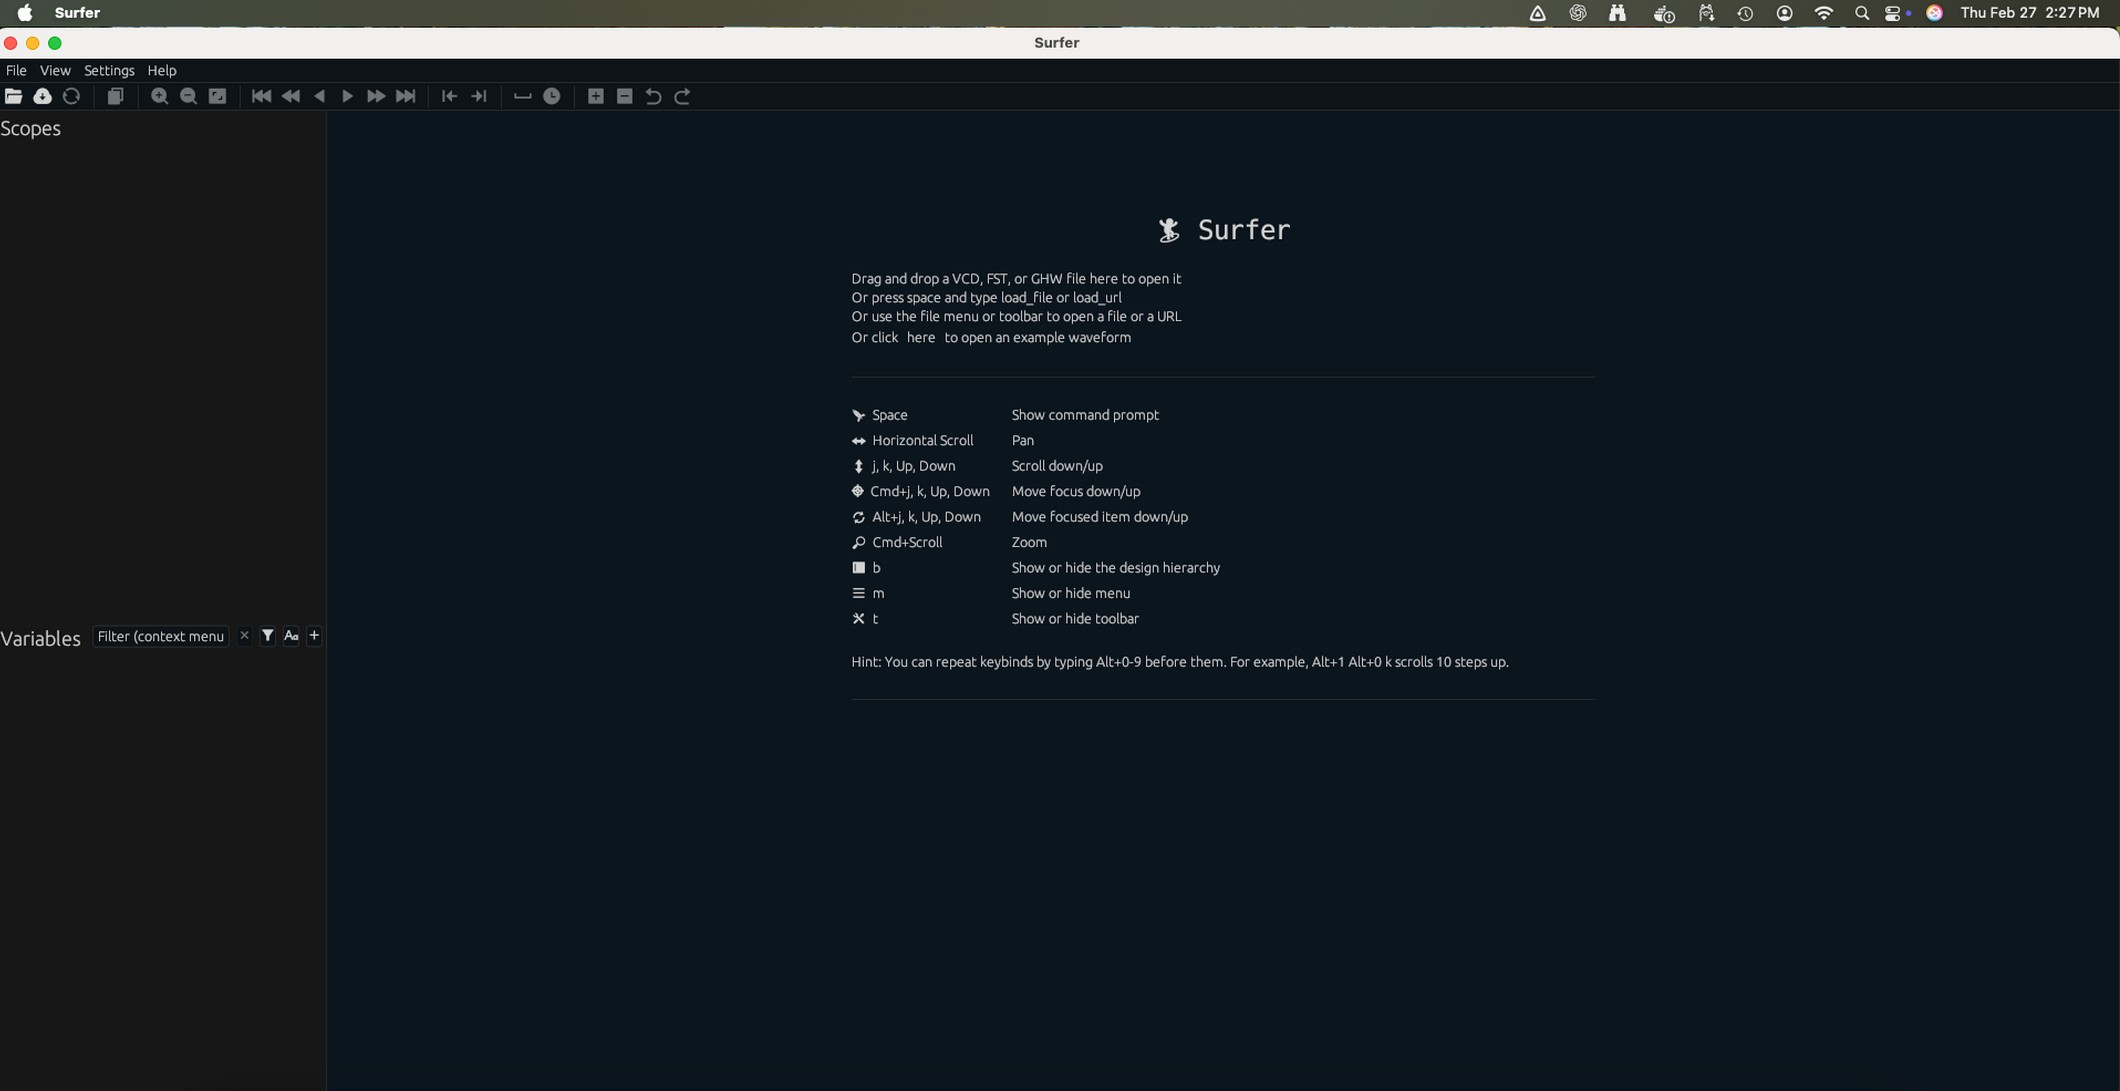
\includegraphics[width=0.8\linewidth]{images/SurferScreenshot.jpg}
    \caption{Surfer Screenshot}
    \label{fig:surfer_screenshot}
\end{figure}

